% Metódy inžinierskej práce

\documentclass[10pt,twoside,slovak,a4paper]{article}

\usepackage[slovak]{babel}
%\usepackage[T1]{fontenc}
\usepackage[IL2]{fontenc} % lepšia sadzba písmena Ľ než v T1
\usepackage[utf8]{inputenc}
\usepackage{graphicx}
\usepackage{url} % príkaz \url na formátovanie URL
\usepackage{hyperref} % odkazy v texte budú aktívne (pri niektorých triedach dokumentov spôsobuje posun textu)
\usepackage{cite}
%\usepackage{times}
\usepackage[nomarginpar, margin=1.7in]{geometry}%margin inconsistency


\pagestyle{headings}

\title{Agilné postupy pri vývoji medicínskeho softvéru\thanks{Semestrálny projekt v predmete Metódy inžinierskej práce, ak. rok 2021/22, vedenie: Ing. Vladimír Mlynarovič PhD.}} 

\author{Irina Makarova\\[2pt]
	{\small Slovenská technická univerzita v Bratislave}\\
	{\small Fakulta informatiky a informačných technológií}\\
	{\small \texttt{xmakarovai@stuba.sk}}
	}

%\date{\small 4. oktober 2021}



\begin{document}
%\renewcommand{\abstractname}{\vspace{-\baselineskip}} %removes abstract heading
\maketitle

\begin{abstract}
V súčasnosti sa rýchlo vyvíja trh zdravotníckych prenositeľných zariadení. Vodopádový model, ktorý sa klasicky používal pri vývoji bezpečnostne kritického softvéru, už pre svoju zdĺhavosť a nepružnosť nepredstavuje optimálny postup. Do popredia sa dostávajú rôzne agilné a kombinované prístupy, čo prináša so sebou otázku, ako implementovať do procesu vývoja agilné metódy a pri tom dodržať požadované normy. Tento článok prináša stručný prehľad aktuálne platných noriem; vysvetľuje podstatu vodopádového a agilných modelov (Scrum, XP, DSDM), porovnáva ich a poukazuje na črty jednotlivých stratégií, ktoré sú prínosné pre túto oblasť. V článku sa uvádzajú niektoré existujúce riešenia, ako sa tieto modely dajú efektívne kombinovať pri vývoji medicínskeho softvéru.
\end{abstract}

\section{Úvod} %dokoncene
S postupným vývojom internetu vecí sa do domácností dostáva čoraz viac zariadení so vstávaným softvérom. V súčasnosti vzrastá dopyt po prenositeľných zdravotníckych pomôckach slúžiacich na monitorovanie alebo korekciu zdravotných problémov. Vývoj softvéru, ktorý je súčasťou týchto zariadení, má prebiehať v súlade s platnými normami. Požiadavky uvedené v normách a smerniciach sú všeobecné a nemožno ich jednoducho nasadiť do praxe. Klasický sekvenčný prístup zdanlivo najlepšie pokrýva všetky rozmanité požiadavky. Dodnes sa väčšina firiem v tejto doméne riadi V-modelom vývoja softvéru\cite{mchugh2013}. Tento postup má však jednu zásadnú nevýhodu – netoleruje zmeny. V rýchlo sa meniacom svete technológií na každom stupni vývoja môže nastať potreba niečo upraviť s ohľadom na nové požiadavky. Okrem toho sa produkt musí rýchlo dostať k užívateľom, aby mal šancu etablovať sa na trhu. 
Agile si osvojili softvérové spoločnosti po celom svete. 84\% respondentov pracujúcich v oblasti softvérového inžinierstva uviedlo, že ich tím využíva nejakú formu agile. Hlavnými príčinami popularity týchto metodík je ich efektívnosť, flexibilnosť a urýchlené dodanie funkčného produktu\cite{agile}. Ich miera adopcie v doméne vývoja bezpečnostné kritických systémov, akým je aj medicínsky softvér, je však stále nízka\cite{mchugh2013}. Jedným z dôvodov je, že agilné postupy sa javia byť v rozpore s regulačnými požiadavkami. Výrobcovia softvéru pre medicínske zariadenia sú pre schválenie produktu povinní predkladať rozsiahlu dokumentáciu, avšak jeden z agilných princípov znie “Funkčný softvér je viac ako vyčerpávajúca dokumentácia“. Aj keď samostatne žiadna z agilných metodík naozaj nie vhodná na vývoj zdravotníckeho softvéru, zavedením istých agilných praktík sa proces vývoja dá zoptimalizovať a lepšie prispôsobiť aktuálnemu stavu prostredia. Hlavným cieľom tohto článku je poukázať na užitočnosť agilných prístupov vo vývoji zdravotníckeho softvéru a vysvetliť na príklade rámca MDevSPICE a agilného V-modelu ako sa klasické a iteratívne modely dajú výhodne kombinovať tak, aby sa vzájomne dopĺňali. 

\section{Normy pre medicínsky softvér}%este doplnim par viet o norme  ISO IEC 62304:2006
Podľa nariadenia o zdravotníckych pomôckach 2017/745 (MDR) sa za zdravotnícku pomôcku považuje akýkoľvek výrobok, ktorý je výrobcom určený na použitie za účelmi ako sú diagnostika, predikcia, sledovanie, prevencia, liečba alebo zmiernenie choroby, a ktorý nedosahuje svoj účinok pomocou farmakologických alebo imunologických prostriedkov. Pod túto definíciu spadá nielen softvér zabudovaný v špecializovaných prístrojoch ale aj softvér ako taký, tzv. SaMD (Software as a Medical Device). Zdravotnícky softvér sa zaraďuje medzi bezpečnostne kritický softvér. To znamená, že jeho nesprávna funkčnosť môže ohroziť zdravie, alebo dokonca život človeka. V závislosti od rizík spojených s jeho používaním sa softvér klasifikuje na tri triedy. Z tejto klasifikácie potom vyplývajú spôsoby, akými sa preukazuje jeho bezpečnosť, a požiadavky, ktoré má spĺňať. V závislosti od regiónu, v ktorom sa má zdravotnícka pomôcka uviesť na trh, sa musia dodržiavať rôzne normy alebo usmernenia. V USA je to Úrad pre kontrolu potravín a liečiv (FDA). Vo všeobecnosti platí, že pri posudzovaní a schvaľovaní zdravotníckych pomôcok v Európskej únii neexistuje žiadny centralizovaný regulačný orgán, ako napríklad Európska agentúra pre lieky (EMA), alebo americký úrad FDA. V EÚ výrobca musí preukázať, že produkt spĺňa platné štandardy. Kľúčovým štandardom pre vývojárov medicínskeho softvéru je ISO IEC 62304:2006\cite{bronneke2021}. Podľa neho musí vývoj softvéru prebiehať podľa vopred stanoveného modelu životného cyklu.

\section{Modely riadenia vývoja softvéru}%dokoncene
Všeobecne sa proces vývoja softvéru dá organizovať dvoma spôsobmi – sekvenčne a iteratívne. Pri tradičnom sekvenčnom vývoji sa najprv zostaví dokument všetkých požiadaviek na softvérový produkt. Na základe neho sa potom navrhne a implementuje produkt. Môže sa však stať, že požiadavky, ktoré zadá zákazník budú nepresné a neúplné, alebo sa pri testovaní v neskorších fázach objaví chyba. Vtedy sa bude treba vracať k predchádzajúcim etapám vývoja softvéru a aplikovať nové požiadavky na návrh, testovanie alebo implementáciu. V dôsledku častých alebo výrazných zmien požiadaviek je potom nutné zvýšiť rozpočet alebo oddialiť termín dodania. Toto zase môže viesť až k nepoužiteľnosti vytvorených softvérových systémov kvôli ich neaktuálnosti. Snaha nájsť alternatívu tomuto postupu vyústila k vzniku množstva techník a metodík, ktoré sa všeobecne volajú agile. Základné princípy agile boli sformulované skupinou 17 vývojárov v roku 2001 a sú zadokumentované v Manifeste pre agilný vývoj softvéru\cite{agileManifesto}, ktorý postuluje nasledujúce: 
\begin{itemize}
\item Ľudia a komunikácia sú viac ako len procesy a nástroje
\item Funkčný softvér je viac ako vyčerpávajúca dokumentácia
\item Spolupráca so zákazníkom je viac ako dojednávanie zmluvy
\item Radšej reagovať na zmenu ako sa držať plánu
\end{itemize}
Dodržiavať tieto hodnoty v praxi umožňuje inkrementálny spôsob vývoja a tesná spolupráca so zákazníkom. Agilné metodiky sú iteratívne – tvorba projektu prebieha v cykloch. Každý cyklus, alebo iterácia, sa dá chápať ako menší projekt, ktorého výstupom je vždy funkčná otestovaná verzia produktu. Výsledkom toho je, že sa k zákazníkovi už po prvých iteráciách dostane prevádzková verzia softvéru, ktorú vie vyskúšať a poskytnúť spätnú väzbu. Prípadné pripomienky zákazníka sa potom stávajú súčasťou nasledujúcej iterácie. Táto prispôsobivosť zmenám a flexibilita požiadaviek má významný dopad na kvalitu produktu a jeho prijatie zákazníkom. 
%nizsie popisane metodiky este budem doplnat

\textbf{V-model} je v oblasti vývoja zdravotníckeho softvéru najpoužívanejším modelom. Je rozšírením vodopádového modelu. Dáva do súvislosti v ňom špecifikované vývojové aktivity s testovacími aktivitami. Pozostáva z dvoch vetiev, ktoré znázorňujú časovú postupnosť jednotlivých etáp vývoja a testovania.

\textbf{Scrum} je predovšetkým spôsob manažmentu, menej sa zaoberá technickou stránkou softvérového inžinierstva. V súčasnosti je najrozšírenejšou agilnou metodikou\cite{agile}. Vývoj podľa scrum prebieha v rámci postupnosti pevne časovo ohraničených cyklov, tzv. sprintov. Po skončení každého z nich má tím byť schopný dodať potenciálne nasaditeľný produkt. Kontrola a prispôsobenie procesu vývoja sa vykonáva počas denných porád a taktiež na konci každého sprintu. Aktivita na projekte sa priebežne zaznamenáva v štyroch hlavných dokumentoch – produktový backlog (zoznam požiadaviek na produkt), sprint backlog (zoznam úloh pre daný sprint), release burndown (sledovanie ešte nerealizovaných položiek produktového backlogu), sprint burndown (sledovanie ešte nerealizovaných položiek v rámci prebiehajúceho sprintu).
Tímy pracujúce podľa scrum sú samo-organizované a obsahujú tri roly - vlastník produktu, scrum master a vývojár. Prácu vývojárskeho tímu usmerňuje scrum master, ktorý slúži ako styčný bod medzi ním a zákazníkom\cite{scrum}.

\textbf{Extrémne programovanie (XP)} je v porovnaní s inými agilnými rámcami pomerne mladá metodika. Jej vznik sa datuje od roku 1999. XP zhrňuje praktiky softvérového inžinierstva tak, aby sa dalo vyvíjať čo najkvalitnejší produkt v udržateľnom čase. Najdôležitejšími z týchto praktík sú: jednoduchý návrh, refaktorizácia, priebežné testovanie funkčných blokov, programovanie v pároch, krátke iterácie, tesná prepojenosť so zákazníkom. Ideový základ XP tvorí päť hodnôt: \emph{jednoduchost} – konať len na základe súčasných požiadaviek zákazníka, nesnažiť sa urobiť to, čo by zákazník mohol chcieť implementovať neskôr, pri návrhu sa riadiť otázkou 'ako vyzerá najjednoduchšie funkčné riešenie?'; \emph{spätná väzba} – zákazník je aktívne zapojený do procesu vývoja, vývoj je riadený testami; \emph{komunikácia a rešpekt} – metodika predpokladá priaznivé podmienky pre spoluprácu, členovia tímu by nemali pracovať samostatne podľa vlastných pravidiel, spoločné vlastnenie kódu, keďže sa na jeho písaní podieľa celý tím, párové programovanie; \emph{odvaha}.

\textbf{Metóda dynamického vývoja systémov} presne definuje postupy a pravidlá vývoja softvéru. Je založená na deviatich princípoch, ktoré by mali byť dodržiavané počas jednotlivých fáz životného cyklu. Vývoj sa riadi tak, aby bol ukončený do stanoveného času a za stanovené prostriedky. DSDM sa menej zaoberá programovacimi prístumi, ale podporuje skôr riadenie projektov. Dá sa kombinovať s inými agilnými metodikami.

\section{Kombinované prístupy}
\textbf{MDevSPICE} je rámec postupov vývoja softvéru pre zdravotnícke pomôcky. Výzva, ktorej čelia spoločnosti vyvíjajúce zdravotnícky softvér, je dodržiavanie veľkého množstva regulačných požiadaviek uvedených v rôznych medzinárodných normách. Tento rámec bol vyvinutý s cieľom pomôcť firmám lepšie sa pripraviť na náročné a nákladné regulačné audity\cite{mccaffery2019}.

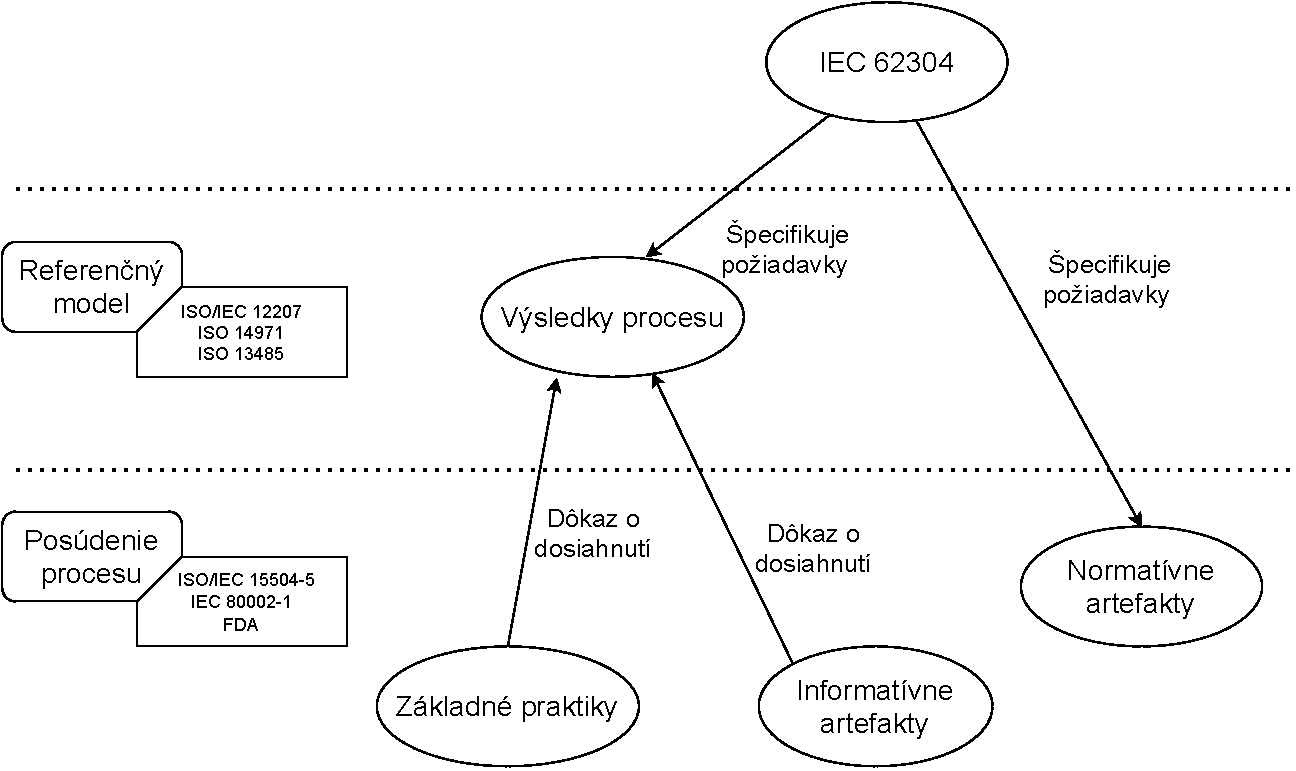
\includegraphics[scale=0.5]{MDevSPICE.pdf}

Obrázok 1. Základné prvky rámca MDevSPICE\cite{ramecmd} - procesný referenčný model a model posudzovania efektívnosti.

Cieľom procesného referenčného modelu MDevSPICE® je poskytnúť komplexný model posúdenia softvéru a procesov vývoja systémov na základe všeobecne uznávaných predpisov o zdravotníckych pomôckach, noriem a smerníc, ktoré má firma zaoberajúca sa vývojom zdravotníckeho softvéru dodržiavať. Daný model, podobne ako ISO/IEC 15504-5 (SPICE), má dve časti - dimenziu procesu a dimenziu spôsobilosti.

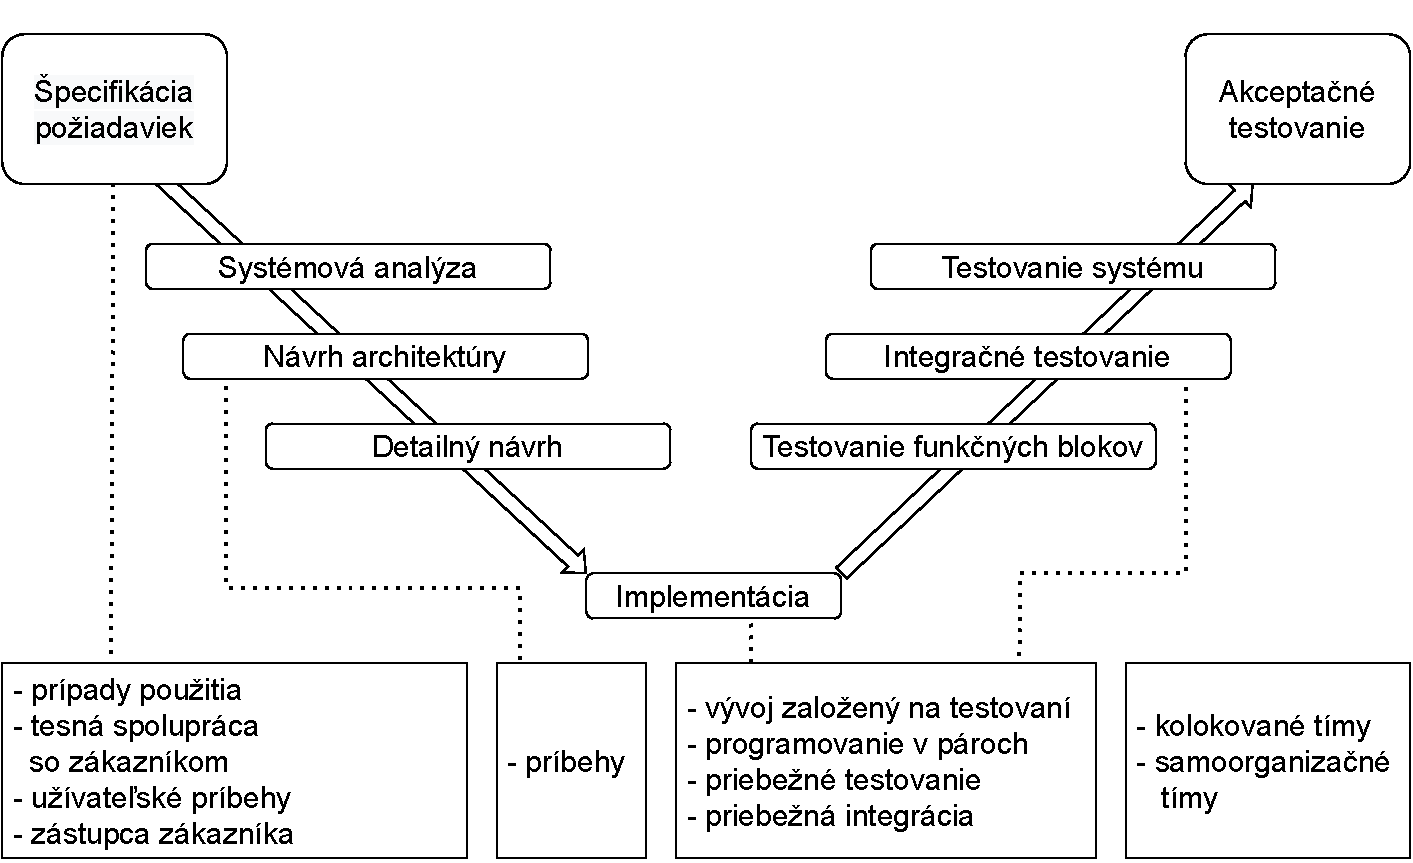
\includegraphics[scale=0.5]{avmodel.pdf}

Obrázok 2. Agilný V-model podľa\cite{mchugh2013}. Prerušovanými čiarami sú spojené agilné praktiky a fázy V-modelu, v ktorých môžu byť použité. Dve praktiky (kolokované a somoorganizačné tímy) sa nevzťahujú na konkrétnu fázu vývoja, ale súvisia skôr so štruktúrou tímu.

\section{Záver}
%Agilný V-model\cite{mchugh2013}
%Agilný V-model

% generuje zoznam literatúry z obsahu súboru literatura.bib
\bibliography{literatura}
\bibliographystyle{plain} % alpha/ abbrv/ plain
\end{document}
